% Template for Cogsci submission with R Markdown

% Stuff changed from original Markdown PLOS Template
\documentclass[10pt, letterpaper]{article}

\usepackage{cogsci}
\usepackage{pslatex}
\usepackage{float}
\usepackage{caption}

% amsmath package, useful for mathematical formulas
\usepackage{amsmath}

% amssymb package, useful for mathematical symbols
\usepackage{amssymb}

% hyperref package, useful for hyperlinks
\usepackage{hyperref}

% graphicx package, useful for including eps and pdf graphics
% include graphics with the command \includegraphics
\usepackage{graphicx}

% Sweave(-like)
\usepackage{fancyvrb}
\DefineVerbatimEnvironment{Sinput}{Verbatim}{fontshape=sl}
\DefineVerbatimEnvironment{Soutput}{Verbatim}{}
\DefineVerbatimEnvironment{Scode}{Verbatim}{fontshape=sl}
\newenvironment{Schunk}{}{}
\DefineVerbatimEnvironment{Code}{Verbatim}{}
\DefineVerbatimEnvironment{CodeInput}{Verbatim}{fontshape=sl}
\DefineVerbatimEnvironment{CodeOutput}{Verbatim}{}
\newenvironment{CodeChunk}{}{}

% cite package, to clean up citations in the main text. Do not remove.
\usepackage{apacite}

% KM added 1/4/18 to allow control of blind submission


\usepackage{color}

% Use doublespacing - comment out for single spacing
%\usepackage{setspace}
%\doublespacing


% % Text layout
% \topmargin 0.0cm
% \oddsidemargin 0.5cm
% \evensidemargin 0.5cm
% \textwidth 16cm
% \textheight 21cm

\title{Children know what words other children know}

\usepackage{booktabs}
\usepackage{longtable}
\usepackage{array}
\usepackage{multirow}
\usepackage{wrapfig}
\usepackage{float}
\usepackage{colortbl}
\usepackage{pdflscape}
\usepackage{tabu}
\usepackage{threeparttable}
\usepackage{threeparttablex}
\usepackage[normalem]{ulem}
\usepackage{makecell}
\usepackage{xcolor}



\begin{document}

\maketitle

\begin{abstract}
To communicate successfully, we need to use words that our
conversational partner understands. Adults maintain precise models of
the words people are likely to know, using both prior experience with
their conversational partner and general metalinguistic information. Do
children also know what words others are likely to know? We asked
children ages 4-8 (\(n =\) 62) to predict whether a very young child
would know each of 15 familiar animal words, all typically acquired
within a 6-month range. With minimal information, even children as young
as 4 made reliable predictions about the target child's vocabulary
knowledge. Further, children's accuracies improved significantly over
the course of development. Thus, even preschool age children are adept
at inferring other children's vocabulary knowledge, and they could
leverage this information to communicate effectively.

\textbf{Keywords:}
communication, metalinguistic, knowledge reasoning, cognitive
development
\end{abstract}

\hypertarget{introduction}{%
\section{Introduction}\label{introduction}}

Imagine visiting the zoo with your friend and their 2-year-old. As you
walk by the peacocks, you hear your friend say, ``Do you see those blue
birds?'' Immediately, you know that your friend is talking to their
child and not you. If they were talking to you, saying ``peacock'' would
be perfectly clear; however, ``blue bird'' might be a better description
for a child who has never seen a peacock before. Even when talking about
the same object, we use different words depending on what we think our
conversational partners know and don't know.

Adults track and adapt to their conversational partners' knowledge with
relative ease. For example, adults reduce the information they give when
re-telling a story to someone who has heard it before, but not when
telling the story to a new partner (Galati \& Brennan, 2010). Adults can
adapt even to partners who are quite different from them, as in the case
of parents and their children. Parents model the fine-grained details of
their children's vocabularies and use these models in spontaneous
communication (e.g., using ``blue bird'' to describe a peacock; Leung,
Tunkel, \& Yurovsky, in press). These vocabulary models are shaped by
extensive individual parent-child interactions, but likely also general
metalinguistic knowledge-- for instance, that shorter words are
typically simpler than longer words and more likely to be known.

In line with this conjecture, Kuperman, Stadthagen-Gonzalez, \&
Brysbaert (2012) asked people to report the age at which they understood
a set of 30,000 English words. They found that adults typically
overestimated the ages at which words are learned, but were quite
accurate at judging their relative order. Thus, even adults without
children have access to the kind of metalinguistic information they
could use to calibrate speech to children's knowledge.

Can children use this same kind of information to predict whether others
will know words? Reasoning about another person's specific lexical
knowledge may prove difficult for young children as they show consistent
errors in reasoning about other's knowledge, commonly over-attributing
knowledge (e.g., Gopnik \& Astington, 1988; Taylor, Esbensen, \&
Bennett, 1994). The bias to over-attribute knowledge is particularly
pronounced for information that the child themselves knows, or is
familiar with (Birch \& Bloom, 2003; Ghrear, Fung, Haddock, \& Birch,
2020).

However, even preschool age children are able to make non-egocentric
knowledge judgments in some tasks. Asked about variety of general
knowledge skills, young children attribute different levels of knowledge
to infants, preschool children, and adults (Fitneva, 2010; Taylor,
Cartwright, \& Bowden, 1991). By at least age 6, children even judge
adults as \emph{less} likely than other children to know about some
topics, such as toys or children's television (Fitneva, 2010;
VanderBorght \& Jaswal, 2009). While these studies sometimes include
vocabulary items among other kinds of knowledge items (e.g., Taylor et
al., 1991), they rely on large scale distinctions, such as an infant not
knowing any words, a child knowing simple words (e.g., \emph{happy}),
and an adult knowing complex words (e.g., \emph{hypochondriac}).

We ask how children infer another child's specific vocabulary knowledge,
and whether they make word-level predictions that are in line with
expected language acquisition. Children at least as young as 5 can make
metalinguistic judgments about their own vocabulary knowledge,
accurately estimating the age and order in which they learned a variety
of words (Walley \& Metsala, 1992). In our study, we introduced 4- to
8-year-old children to a younger fictional child, and asked them to make
judgments about the target child's knowledge of various familiar words.
The accuracy of children's judgments improved reliably from 4- to
8-years of age, but even 4-year-old children showed knowledge about the
words that the target child was likely to know. We end by discussing
children's own explanations for why the target child would know (or not
know) particular words.

\hypertarget{method}{%
\section{Method}\label{method}}

\hypertarget{stimuli}{%
\subsection{Stimuli}\label{stimuli}}

Our stimuli consisted of 15 words drawn from a single domain (animal
words), along with corresponding images of each animal. We pulled all
animal images (\(n =\) 45) from a normed image set (Rossion \& Pourtois,
2004; recoloring of Snodgrass \& Vanderwart, 1980). To ensure our
stimuli set spanned a range of ages of acquisition (AoAs), we ranked the
animal words from earliest to latest AoA, using adult estimates from
Kuperman et al. (2012), and split the words into five bins. In order to
select animal images that are recognizable and typically identified by a
single name, we chose the three animals from each AoA bin with the
highest naming agreement according to a naming task with children
(Cycowicz, Friedman, Rothstein, \& Snodgrass, 1997).

The resulting animal words, ordered by estimated AoA, were \emph{dog},
\emph{duck}, \emph{cat}, \emph{pig}, \emph{fish}, \emph{turtle},
\emph{zebra}, \emph{elephant}, \emph{snake}, \emph{penguin},
\emph{gorilla}, \emph{owl}, \emph{raccoon}, \emph{leopard}, and
\emph{lobster.} Although adult AoA estimates for these words range from
2.5 to 7.5 years old (Kuperman et al., 2012), all of these animal words
are generally acquired by age 3 according to parent reports of
children's vocabulary knowledge (Frank, Braginsky, Yurovsky, \&
Marchman, 2017). Because the youngest children in our study are 4 years
old, we expected all participants to know these animal words.

\hypertarget{participants}{%
\subsection{Participants}\label{participants}}

We pre-registered a planned sample of 60 children ages 4-8, with 12
children recruited for each year-wise age group. Due to overrecruitment,
our final sample included 62 children (12 4-year-olds, 13 5-year-olds,
13 6-year-olds, 12 7-year-olds, 12 8-year-olds). All analyses hold when
looking only at the 60 children run first chronologically. Based on a
pre-registered exclusion criterion, children who failed to answer all of
the questions were excluded and replaced (an additional 6 children).
Families were recruited online, primarily through a US University
database of families who have expressed interest in doing research or
previously participated. Children completed this study over Zoom,
interacting with a live experimenter who navigated a slide-style,
animated Qualtrics survey.

A separate sample of 30 adults were recruited via Amazon Mechanical
Turk. The adult sample provides a simple test that our task elicits
robust inferences about the target child's lexical knowledge, and that
these inferences correspond to extant AoA data. Adult participants
completed the same task using Qualtrics, with minor modifications as
described below.

\hypertarget{procedure}{%
\subsection{Procedure}\label{procedure}}

\begin{CodeChunk}
\begin{figure}[tb]

{\centering 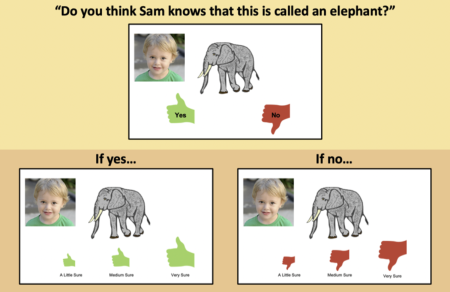
\includegraphics{figs/task-method-1} 

}

\caption[The structure of an example trial]{The structure of an example trial. The experimenter labeled the animal, then asks the child “Do you think Sam knows that this is called an elephant?” Based on their response, children were then asked to provide a confidence judgment on a 3-point scale (little sure, medium sure, very sure).}\label{fig:task-method}
\end{figure}
\end{CodeChunk}

\emph{Introduction.} Children were shown a picture of a child named
``Sam'' (seen in Figure \ref{fig:task-method}). Children were anchored
to Sam's knowledge of various familiar skills, specifically some skills
that Sam has acquired (e.g., coloring), and some that Sam has not yet
acquired (e.g., reading). Children were then specifically anchored to
Sam's possible word knowledge in an unrelated domain--given an example
of one word Sam knows (\emph{car}), and one word that Sam does not know
(\emph{piano}). This introduction was intended to familiarize the
children with Sam, roughly anchor them to Sam's knowledge and age, and
to ensure that children understand there are things Sam does \emph{not}
know yet (even things children themselves likely know, such as how to
read).

\emph{Trial structure.} On each trial, children were shown a drawing of
a familiar object or animal (Rossion \& Pourtois, 2004). The
experimenter first labeled the object (e.g., ``Look, it's {[}an
elephant{]}!''), and then asked about the target child's knowledge
(e.g., ``Do you think Sam knows that this is called {[}an elephant{]}?
Yes or no?''). Based on their response, children were then asked a
follow-up question: ``How sure are you that Sam {[}knows/doesn't know{]}
that this is called {[}an elephant{]}--a little sure, medium sure, or
very sure?'' All questions were presented with accompanying pictures of
thumbs {[}up/down{]} of varying size (see Figure \ref{fig:task-method}).
Children as young as 3 are able to engage in uncertainty monitoring and
report their confidence, although these skills do develop in the
preschool years (Lyons \& Ghetti, 2011). Children's responses to these
two items were recoded onto a 1-6 scale from 1--\emph{very sure Sam
doesn't know} to 6--\emph{very sure Sam knows}.

The experimenter provided no evaluative feedback on any trials, but did
offer consistent neutral feedback (e.g., repeating the child's answer or
saying ``Okay!''). When a child failed to respond within about 5 seconds
or offered a non-canonical response (e.g., saying ``Maybe''), the
experimenter acknowledged the child's answer and then repeated the
question with the possible responses. If a child did not answer after
the question was repeated, the experimenter moved on and marked the
trial as no response. These were considered ``incomplete'' sessions and
these participants were not included in the final sample.

\emph{Familiarization trials.} Children first completed two non-animal
familiarization trials, one for an early-acquired word (\emph{ball}) and
one for a late-acquired word (\emph{artichoke}). These trials followed
the trial structure described above and were intended to help
familiarize children with the structure of the questions and scales.
These trials were always asked first and in a fixed order.

\emph{Animal trials.} Children were then shown 15 trials of the same
form (see example trial in Figure \ref{fig:task-method}). For the 15
animal trials, trial order was randomized across participants to control
for any potential order effects in children's responses.

\emph{Explanation.} After completing the final animal trial, children
were asked an open-ended explanation question about their final judgment
(e.g., ``Why do you think Sam {[}knows/doesn't know{]} that this is
called {[}an elephant{]}?''). Because the trial order was randomized,
the explanations concerned different animal words across participants.

\emph{Final check questions.} Children were asked two questions about
Sam's skill knowledge, one early-acquired skill (\emph{going up and down
stairs}) and one very late-acquired skill (\emph{driving a car}). These
questions again followed the general trial structure described above.
The skill knowledge items were included as an additional check that
children at all ages were able to use the scale appropriately, in case
young children failed to differentiate animal words based on AoA.
Lastly, children were asked to report how old they thought Sam was. This
question was intended to assess another aspect of children's belief
about Sam. Sam's photo and skill knowledge were intended to indicate
toddlerhood.

\hypertarget{adult-procedure.}{%
\paragraph{Adult procedure.}\label{adult-procedure.}}

Adult participants completed a minimally adapted version of the same
task online via Qualtrics. Unlike children, adults were simply presented
with the full 6-point scale (1--\emph{very sure Sam doesn't know} to
6--\emph{very sure Sam does know}). Additionally, the task was
administered asynchronously, so adult participants did not interact with
an experimenter or receive any feedback during the task. Otherwise, the
adult task was identical to the child task described above.

\begin{CodeChunk}
\begin{figure}[tb]
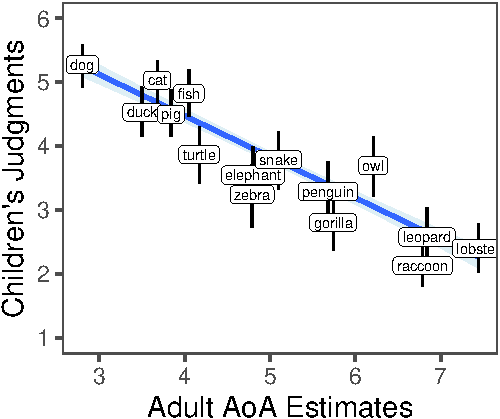
\includegraphics{figs/overall-1} \caption[Comparing adult AoA estimates (in years, taken from Kuperman et al., 2012) and children’s judgments on our 6-point scale (1 = very sure Sam doesn’t know]{Comparing adult AoA estimates (in years, taken from Kuperman et al., 2012) and children’s judgments on our 6-point scale (1 = very sure Sam doesn’t know; 6 = very sure Sam knows). The black lines show 95\% confidence intervals for each item. The shaded region shows the confidence interval based on a linear regression estimated from the raw data.}\label{fig:overall}
\end{figure}
\end{CodeChunk}

\hypertarget{results}{%
\section{Results}\label{results}}

\hypertarget{familiarization-trials}{%
\subsection{Familiarization trials}\label{familiarization-trials}}

Children completed two familiarization trials asking about the target
child's knowledge of two non-animal words (\emph{ball} and
\emph{artichoke}). These questions were primarily included to help
children get accustomed to the general trial structure. To analyze
children's responses on these familiarization items, we used a mixed
effects model using the \texttt{lme4} package in \texttt{R} (Bates,
Mächler, Bolker, \& Walker, 2015), predicting children's knowledge
judgments from the item with a random effect of participant.

Overall, children were significantly more likely to report that Sam
knows the word \emph{ball} (\(mean =\) 4.65) than that Sam knows the
word \emph{artichoke} (\(mean =\) 1.87, \(\beta =\) 2.77, \(t =\) 10.6,
\(p =\) \textless{} .01). Analyzing judgments separately for each age
group, 4-year-olds did not significantly differentiate the two
familiarization items (\(\beta =\) 0.17, \(t =\) 0.21, \(p =\) .83). All
other age groups significantly differentiated the two familiarization
items (\(ps <\) 0.05).

\hypertarget{skill-knowledge}{%
\subsection{Skill knowledge}\label{skill-knowledge}}

We also included two questions about the target child's skill knowledge.
These questions were intended primarily as a check that children at all
ages were able to use the scale appropriately and able to infer
knowledge in an easier case. Note that the two skill items (\emph{going
up and down stairs}, and \emph{driving a car}) are in line with
children's own knowledge, unlike the animal word items. That is, child
participants should be able to answer these questions appropriately even
if they are reasoning egocentrically about their own knowledge.

Overall, children differentiated the target child's skill knowledge on
these two items. We used a similar mixed effects structure predicting
children's knowledge judgments from the item and a random effect of
participant. Children were significantly more likely to report that the
target child knows how to go up and down stairs (\(mean =\) 4.1) than
that the child knows how to drive a car (\(mean =\) 1.4, \(\beta =\)
2.69, \(t =\) 10.29, \(p =\) \textless{} .01). Analyzing judgments
separately for each age group, even 4-year-olds significantly
differentiated the two skill items (\(\beta =\) 2.33, \(t =\) 4.31,
\(p =\) \textless{} .01).

\begin{CodeChunk}
\begin{figure*}[tb]
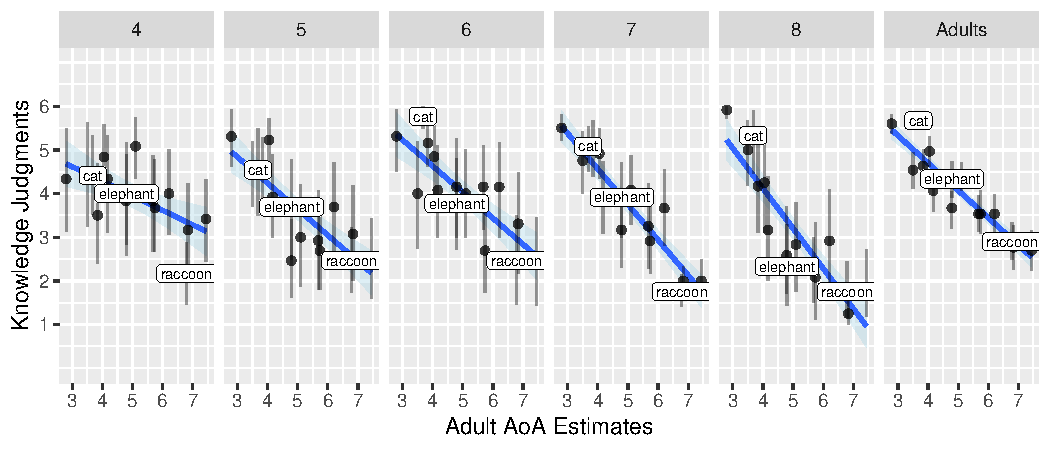
\includegraphics{figs/development-1} \caption[Children and adults judgements about the target child's word knowledge across development, compared with adult AoA estimates (in years, taken from Kuperman et al., 2012)]{Children and adults judgements about the target child's word knowledge across development, compared with adult AoA estimates (in years, taken from Kuperman et al., 2012). Each point represents 1 of the 15 word items, with black lines showing 95\% percent confidence intervals for each item. The shaded region shows the confidence interval based on a linear regression estimated from the raw data.}\label{fig:development}
\end{figure*}
\end{CodeChunk}

\hypertarget{judgments-of-vocabulary-knowledge}{%
\subsection{Judgments of vocabulary
knowledge}\label{judgments-of-vocabulary-knowledge}}

Our primary analyses compare knowledge judgments on our 6-point scale to
AoA judgments from adults (taken from Kuperman et al., 2012). Data were
analyzed using a pre-registered mixed effects model. We predicted
children's judgments from adult AoA estimates, including random effects
for participant and word.

We expected that overall, children's judgments would recover the ordinal
shape of age of acquisition data for these items. That is, children
would infer that the target child is most likely to know early-acquired
words, and least likely to know late-acquired words. As a result, we
expected a negative relationship between judgments of the target child's
lexical knowledge and adult AoA estimates.

First, analyzing adults responses on our task, we saw the predicted
negative correlation between AoA and adults' judgments of the target
child's knowledge (Figure \ref{fig:development}, \(\beta =\) -0.63,
\(t =\) -8.71, \(p\) \textless{} .01). This confirmed that our task
elicited reliable predictions from adults, and that adults' inferences
about the target child's knowledge match predictions from AoA estimation
tasks (Kuperman et al., 2012).

Do children's judgments about another child's vocabulary knowledge also
reflect a sensitivity to which words are learned earlier or later?
Overall, we found a significant negative effect of AoA on children's
judgments (\(\beta =\) -0.65, \(t =\) -8.29, \(p\) \textless{} .001). As
a group, children judged that the target child would be most likely to
know an early-acquired word (e.g., dog) and least likely to know a
late-acquired word (e.g., lobster, see Figure \ref{fig:overall}).

We then asked whether children develop sensitivity to Sam's vocabulary
knowledge, with older children's judgments recovering word-level AoA
data more closely. We used the same mixed effects model but included an
effect of age and an interaction between AoA and age. We again found a
reliable main effect of AoA (\(\beta =\) -0.65, \(t =\) -8.29, \(p\)
\textless{} .001), a main effect of age (\(\beta =\) 0.55, \(t =\) 3.68,
\(p\) \textless{} .001) and a significant interaction between the two
(\(\beta =\) -0.14, \(t =\) -5.1, \(p\) \textless{} .001). Thus, as
predicted, we observed that older children judged whether Sam would know
each animal in a more adult-like, and more accurate, way (Figure
\ref{fig:development}).

\begin{CodeChunk}
\begin{figure}[tb]
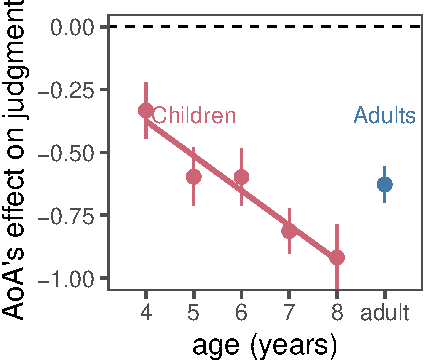
\includegraphics{figs/age_terms-1} \caption[Coefficient estimates of the effect of age acquisition on children's and adults' knowledge judgments]{Coefficient estimates of the effect of age acquisition on children's and adults' knowledge judgments. Points indicate means, error bars indicate 1 SD.}\label{fig:age_terms}
\end{figure}
\end{CodeChunk}

To test the robustness of this intuition at each age, we ran the model
separately for each pre-determined year-wise age group (Figure
\ref{fig:age_terms}). We found a significant negative correlation
between AoA and children's judgments at all age groups (with the
smallest effect in 4-year-olds: \(\beta =\) -0.33, \(t =\) -3.01,
\(p =\) .01). That is, even 4-year-old children judged that
late-acquired animal words were less likely to be known by the target
child. Interestingly, the older two age-groups of children were more
accurate than adults in judging Sam's knowledge (Figure
\ref{fig:age_terms}). This appeared to be primarily driven by a greater
willingness to judge Sam as moderately or very unlikely to know
late-learned animal words, whereas adults were less sure about these
same judgments (Figure \ref{fig:development}). We return to this finding
in the Discussion.

\hypertarget{how-old-is-the-target-child}{%
\subsection{How old is the target
child?}\label{how-old-is-the-target-child}}

At the end of the study, participants were asked to guess the target
child's age. While the familiarization phase included information about
the child's language and skill knowledge, no age was explicitly given.
Looking at children's responses, the median response was that the target
child was 3-years-old. Looking at adult's responses, the median response
was that the target child was 4-years-old.

\hypertarget{explanations}{%
\subsection{Explanations}\label{explanations}}

\begin{table*}[tb]
\centering
\begin{tabular}{ll}
  \hline
Category & Example Utterance \\ 
  \hline
Language & Because it was a very long word. \\ 
    & Because it only has 3 letters. \\ 
  Experience & Because maybe he has a dog. \\ 
    & Because gorillas are really rare animals \\ 
  Location & Because penguins live in the arctic and it's too cold for little kids... \\ 
    & Because fish swim under the ocean. \\ 
  Age & Because I think I knew that when I was around 3... \\ 
    & Because if he went to preschool then he probably knew it... \\ 
  Unsure & I don't know. \\ 
    & I'm not sure. \\ 
  Other & Because it had a longer beak than a bird. \\ 
    & Because it's small. \\ 
   \hline
\end{tabular}
\caption{Example explanations from child participants for each of the five categories used for coding.} 
\label{tab:explanations_table}
\end{table*}

As an exploratory analysis, we examined the reasons young children gave
for why the target child would or would not know a given word. While
children sometimes offered spontaneous explanations throughout the
study, this analysis focuses on the explanation elicited after the final
animal trial. The explanations were divided into 6
non-mutually-exclusive categories: \emph{Language}, \emph{Experience},
\emph{Location}, \emph{Age}, \emph{Unsure}, and \emph{Other}.

\emph{Language} includes explanations that explicitly appealed to
language properties. \emph{Experience} includes explanations that appeal
to the child's real-world experience with the referent. \emph{Location}
includes explanations that specifically reference a particular place the
animal is associated with. \emph{Age} includes explanations that
reference a particular age or general age-group. Any child that failed
to answer the explanation question or expressed ignorance was coded as
giving an explanation of \emph{Unsure}. An explanation that didn't fall
into any of the above categories was coded as \emph{Other}. Note that
coding was not mutually-exclusive, so explanations could be coded as
including multiple categories. See Table \ref{tab:explanations_table}
for examples of each category. Figure \ref{fig:explanations} shows the
proportion of children who gave each type of explanation.

\begin{CodeChunk}
\begin{figure}[tb]
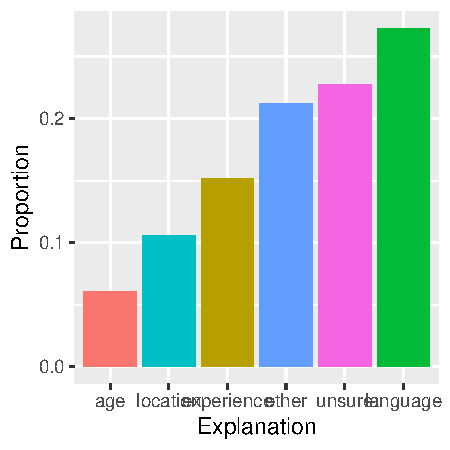
\includegraphics{figs/explanations-1} \caption[Children's explanations for why they think the target child knew or didn't know an animal]{Children's explanations for why they think the target child knew or didn't know an animal. Categories are not mutually exclusive.}\label{fig:explanations}
\end{figure}
\end{CodeChunk}

To understand how children's explanations may change over development,
we divided participants into older (6-8 years old) and younger children
(4-5 years old). Unsurprisingly, \emph{Unsure} explanations were much
more common in younger children (44\%) when compared to older children
(8.33\%). \emph{Language} explanations were used by the highest
proportion of children overall (27.27\%). Do older children account for
all of those explanations? Although more of the older children appealed
to \emph{Language} explanations (30.56\%), these explanations were also
common in younger children (24\%). Thus, while young children were more
likely to offer no explanation, the explanations they did offer seemed
to rely on factors similar to older children's explanations.

\hypertarget{discussion}{%
\section{Discussion}\label{discussion}}

Our ability to infer other people's knowledge is crucial for successful
communication. Young children are capable of inferring others' general
knowledge states, but do they make accurate judgments about another
person's specific knowledge? We asked 4- to 8-year-old children to
estimate another child's knowledge of animal words, and found that
children as young as 4 are sensitive to a younger child's vocabulary
knowledge.

Our findings highlight that young children have robust metalinguistic
knowledge (Walley \& Metsala, 1992), and can use that knowledge to make
highly specific inferences about other people's knowledge. The animal
words used in our study are generally learned within a 6-month period,
yet young children still distinguished early-acquired words from
late-acquired words in this set. Prior studies have demonstrated that
children distinguish the general knowledge of infants, young children,
and adults-- including some vocabulary knowledge items (Fitneva, 2010;
Taylor et al., 1991). Our study further demonstrates that children
readily make specific, word-level predictions about the language
knowledge of another child.

Surprisingly, responses from the oldest children in our sample more
closely correlated with adult judgments of AoA (Kuperman et al., 2012)
when compared to adult participants in this study. This difference
appears to be driven by older children in our study being more likely to
judge that a young child would \emph{not} know late-acquired words. It
is possible that children may be more accurate at estimating other
children's lexical knowledge because of their proximity to the age that
they learned a word (see also Walley \& Metsala, 1992). However, such an
account should also predict that younger children would perform better
than older children when making these inferences, which is counter to
our developmental findings. Additionally, children and adults' estimates
for the target child's age may be an important factor. In our sample,
adults gave higher estimates for the target child's age than children
did, and may have attributed more knowledge to the child more as a
result.

How are children in our study making estimates about other people's
knowledge? Children's own explanations suggest that they use various
cues to make their estimates. Overall, language-related explanations
were most common, and even preschool age children appealed to this
explanation. However, such explanations are difficult to interpret, and
the mechanisms underlying children's knowledge estimates are outside the
scope of the current study. Future work should more directly probe the
features underlying this inference-- to see if children are relying on
their own uncertainty, word length (and other linguistic cues), features
of the referent itself, or other features.

The current work lays the foundation for future research on how children
leverage their knowledge of other people to communicate successfully.
While some studies have found that young children struggle in a variety
of communicative tasks (e.g.~Krauss \& Glucksberg, 1977), other work has
shown that by age 5, children selectively talk about general or specific
characteristics of an object based on their partners' knowledge state
(Baer \& Friedman, 2018). Why might children struggle in some situations
and not others? Our work can begin to address this question by mapping
out whether communicative difficulties stem from tracking an
interlocutor's knowledge, or problems using that information in language
production. Young children eventually become effective communicators,
and our work demonstrates that by age 4 children may have one key
ability in place: inferring others' specific vocabulary knowledge.

\vspace{1em} \fbox{\parbox[b][][c]{7.3cm}{\centering Stimuli, data, and analysis code available after deanonymization.}}

\hypertarget{references}{%
\section{References}\label{references}}

\setlength{\parindent}{-0.1in} 
\setlength{\leftskip}{0.125in}

\noindent

\hypertarget{refs}{}
\leavevmode\hypertarget{ref-baer2018}{}%
Baer, C., \& Friedman, O. (2018). Fitting the message to the listener:
Children selectively mention general and specific facts. \emph{Child
Development}, \emph{89}(2), 461--475.

\leavevmode\hypertarget{ref-bates2015}{}%
Bates, D., Mächler, M., Bolker, B., \& Walker, S. (2015). Fitting linear
mixed-effects models using lme4. \emph{Journal of Statistical Software},
\emph{67}(1), 1--48.

\leavevmode\hypertarget{ref-birch2003}{}%
Birch, S. A., \& Bloom, P. (2003). Children are cursed: An asymmetric
bias in mental-state attribution. \emph{Psychological Science},
\emph{14}(3), 283--286.

\leavevmode\hypertarget{ref-cycowicz1997}{}%
Cycowicz, Y. M., Friedman, D., Rothstein, M., \& Snodgrass, J. G.
(1997). Picture naming by young children: Norms for name agreement,
familiarity, and visual complexity. \emph{Journal of Experimental Child
Psychology}, \emph{65}(2), 171--237.

\leavevmode\hypertarget{ref-fitneva2010}{}%
Fitneva, S. A. (2010). Children's representation of child and adult
knowledge. \emph{Journal of Cognition and Development}, \emph{11}(4),
458--484.

\leavevmode\hypertarget{ref-frank2017}{}%
Frank, M. C., Braginsky, M., Yurovsky, D., \& Marchman, V. A. (2017).
Wordbank: An open repository for developmental vocabulary data.
\emph{Journal of Child Language}, \emph{44}(3), 677--694.

\leavevmode\hypertarget{ref-galati2010}{}%
Galati, A., \& Brennan, S. E. (2010). Attenuating information in spoken
communication: For the speaker, or for the addressee? \emph{Journal of
Memory and Language}, \emph{62}(1), 35--51.

\leavevmode\hypertarget{ref-ghrear2020}{}%
Ghrear, S., Fung, K., Haddock, T., \& Birch, S. A. (2020). Only familiar
information is a ``curse'': Children's ability to predict what their
peers know. \emph{Child Development}.

\leavevmode\hypertarget{ref-gopnik1988}{}%
Gopnik, A., \& Astington, J. W. (1988). Children's understanding of
representational change and its relation to the understanding of false
belief and the appearance-reality distinction. \emph{Child Development},
26--37.

\leavevmode\hypertarget{ref-krauss1977}{}%
Krauss, R. M., \& Glucksberg, S. (1977). Social and nonsocial speech.
\emph{Scientific American}, \emph{236}(2), 100--105.

\leavevmode\hypertarget{ref-kuperman2012}{}%
Kuperman, V., Stadthagen-Gonzalez, H., \& Brysbaert, M. (2012).
Age-of-acquisition ratings for 30,000 english words. \emph{Behavior
Research Methods}, \emph{44}(4), 978--990.

\leavevmode\hypertarget{ref-leung2021}{}%
Leung, A., Tunkel, A., \& Yurovsky, D. (in press). Parents fine-tune
their speech to children's vocabulary knowledge. \emph{Psychological
Science}.

\leavevmode\hypertarget{ref-rossion2004}{}%
Rossion, B., \& Pourtois, G. (2004). Revisiting Snodgrass and
Vanderwart's object pictorial set: The role of surface detail in
basic-level object recognition. \emph{Perception}, \emph{33}, 217--236.

\leavevmode\hypertarget{ref-snodgrass1980}{}%
Snodgrass, J. G., \& Vanderwart, M. (1980). A standardized set of 260
pictures: Norms for name agreement, image agreement, familiarity, and
visual complexity. \emph{Journal of Experimental Psychology: Human
Learning and Memory}, \emph{6}(2), 174.

\leavevmode\hypertarget{ref-taylor1991}{}%
Taylor, M., Cartwright, B. S., \& Bowden, T. (1991). Perspective taking
and theory of mind: Do children predict interpretive diversity as a
function of differences in observers' knowledge? \emph{Child
Development}, \emph{62}(6), 1334--1351.

\leavevmode\hypertarget{ref-taylor1994}{}%
Taylor, M., Esbensen, B. M., \& Bennett, R. T. (1994). Children's
understanding of knowledge acquisition: The tendency for children to
report that they have always known what they have just learned.
\emph{Child Development}, \emph{65}(6), 1581--1604.

\leavevmode\hypertarget{ref-vanderborght2009}{}%
VanderBorght, M., \& Jaswal, V. K. (2009). Who knows best? Preschoolers
sometimes prefer child informants over adult informants. \emph{Infant
and Child Development: An International Journal of Research and
Practice}, \emph{18}(1), 61--71.

\leavevmode\hypertarget{ref-walley1992}{}%
Walley, A. C., \& Metsala, J. L. (1992). Young children's
age-of-acquisition estimates for spoken words. \emph{Memory \&
Cognition}, \emph{20}(2), 171--182.

\bibliographystyle{apacite}


\end{document}
